\chapter{System Design and Architecture}
\markboth{Chapter 3. System Design and Architecture}{Chapter 3. System Design and Architecture}

\section{Introduction}
To bridge the gap between conversational agility and deterministic network infrastructure management, a robust architectural foundation is required. This chapter details the conceptual, structural, and detailed design of our hybrid network orchestration prototype. We translate the theoretical principles of Intent-Based Networking (IBN) established in RFC 9315~\cite{rfc9315} into a concrete software design, isolating the probabilistic natural language processing plane from the deterministic control plane. By grounding our validation rules in classical firewall policy anomaly analysis models such as those proposed by Al-Shaer and Hamed~\cite{alshaer2004discovery} and Yuan et al.~\cite{yuan2006fireman}, we ensure that the hybrid system remains mathematically sound, secure, and fail-safe.

We begin by specifying the functional and non-functional requirements that govern system safety, functionality, and operational performance. We then present the multi-layered block architecture, illustrating the hard trust boundary separating untrusted AI models from verified execution modules. Next, we detail the NLP and RAG Ingestion Pipeline, showcasing the dynamic classifier and semantic vector database enrichment. Finally, we analyze the translation and execution engine, the security compliance safety gates, the transactional state snapshot-rollback lifecycle, and the structural UML models mapping actor interactions and object-oriented class relationships.

\subsection{Transition from Theoretical Frameworks to Architecture}
The theoretical paradigms analyzed in Chapter 2---ranging from declarative Intent-Based Networking (IBN) models to Human-in-the-Loop (HITL) control mechanisms---establish the conceptual requirements for our prototype. However, operationalizing these concepts on physical enterprise hardware requires a concrete software design. This section bridges the theoretical demand for validation gates and trust boundaries with the multi-tiered software architecture described below, detailing our routing modules, grounding engines, session state transition matrices, and UML class designs.

\section{System Requirements and Specifications}
Before translating design principles into software components, we define the strict specifications that govern the system.

\subsection{Functional Requirements}
The functional requirements represent the core capabilities that the orchestrator must perform to assist the network administrator. They are structured into four main operational pillars:
\begin{enumerate}
    \item \textbf{Conversational Interpretation (Read/Write Parsing):} The system must ingest unstructured administrative prompts in English or French, classifying them dynamically into read queries (status, logs, active states) or configuration write intents (policy mutations, object management, system tasks).
    \item \textbf{Contextual Entity Grounding:} The system must dynamically reconcile ambiguous user references (e.g., ``allow public traffic to the mail server'') with active, physical device elements retrieved via live REST API queries (mapping ``mail server'' to its corresponding IP address object and UUID).
    \item \textbf{Deterministic Safety Validation:} The system must perform forward-looking compliance checks, verifying that no policy violates predefined corporate standards (e.g., blocking HTTP/Telnet management or preventing public exposure of insecure ports).
    \item \textbf{Transactional Lifecycle Management:} Before mutating device states, the system must take a complete, localized configuration snapshot. Post-execution, it must verify the active configuration on the physical firewall. If verification fails or communication is severed, the system must automatically execute an inverse rollback to restore the firewall to its pre-state.
\end{enumerate}

\subsection{Non-Functional Requirements}
Non-functional requirements specify the architectural constraints, quality standards, and safety bounds of the implementation:
\begin{itemize}
    \item \textbf{Predictability and Safety:} No configuration modification may be executed directly by a probabilistic model. The AI-assisted interface is strictly restricted to intent parsing, leaving all execution, validation, and API interactions to deterministic Python logic.
    \item \textbf{Operator Oversight (HITL):} All state-mutating transactions require explicit administrative approval. The system must present a side-by-side unified delta diff of the planned changes before requesting confirmation.
    \item \textbf{Auditability and Log Integrity:} Every session interaction, intermediate intent, validation outcome, and API mutation must be recorded in an audit ledger using a rolling SHA-256 hash sequence to detect unauthorized modifications.
    \item \textbf{Latency and Responsiveness:} The intent classification and parsing pipeline must execute within a low-latency threshold, ensuring that typical query resolutions complete in under three seconds to prevent administrator operational delay.
\end{itemize}

\section{Global System Architecture}
The core design principle of our system is the strict, multi-layered segregation of responsibilities, directly addressing the limitations of unconstrained language models highlighted in NetConfEval~\cite{wang2024netconfeval}. We partition the application into two isolated logical zones: the \textbf{Probabilistic Interpretation Plane} (leveraging NLU models and semantic vector indexes) and the \textbf{Deterministic Control Plane} (implemented strictly in Python code using deterministic schemas).

This structural segregation is illustrated in Figure~\ref{fig:trust_boundary_arch}.

\begin{figure}[H]
    \centering
    \makebox[\textwidth][c]{
    \begin{tikzpicture}[
        scale=0.78, every node/.style={transform shape, font=\sffamily\small},
        blockprob/.style={rectangle, draw=blue!70!black, thick, fill=blue!3, text width=3.0cm, align=center, minimum height=1.2cm, rounded corners},
        blockdet/.style={rectangle, draw=green!60!black, thick, fill=green!3, text width=3.0cm, align=center, minimum height=1.2cm, rounded corners},
        database/.style={cylinder, draw=purple!70!black, thick, fill=purple!3, text width=2.0cm, align=center, minimum height=1.3cm, aspect=0.22, shape border rotate=90},
        firewall/.style={cylinder, draw=orange!80!black, thick, fill=orange!3, text width=2.0cm, align=center, minimum height=1.3cm, aspect=0.22, shape border rotate=90},
        arrow/.style={->, thick, draw=black, >=stealth},
        doublearrow/.style={<->, thick, draw=black, >=stealth},
        boundary/.style={draw=red!70, dashed, ultra thick, fill=red!3, fill opacity=0.05, rounded corners}
        ]
        
        % Probabilistic Zone (Blue Theme)
        \node[blockprob] (user) at (0, 0) {User Natural\\Language Prompt};
        \node[blockprob] (router) at (4.8, 0) {Dynamic Classifier\\(agent/router.py)};
        \node[database] (chroma) at (4.8, 2.6) {Vector Database\\(ChromaDB RAG)};
        \node[blockprob] (nlu) at (9.6, 0) {NLU Interpreter\\(nlu\_interpreter.py)};
        
        % Red Gutter dividing the Trust Boundary (Drawn behind the labels)
        \draw[red!80, dashed, ultra thick] (12.0, 3.6) -- (12.0, -5.8);
        \node[fill=white, inner sep=2pt, rotate=270, text=red!80, font=\sffamily\scriptsize\bfseries] at (12.0, 0.8) {HARD TRUST BOUNDARY};
        
        % Deterministic Zone (Green/Orange Theme)
        \node[blockdet] (ground) at (14.4, 0) {Entity Grounder\\(nlu\_grounder.py)};
        \node[blockdet] (val) at (14.4, -2.6) {Safety \& Compliance\\(compliance.py)};
        \node[blockdet] (hitl) at (4.8, -2.6) {HITL Portal\\(streamlit\_app.py)};
        \node[blockdet] (exec) at (0, -2.6) {Transactional Executor\\(executor.py)};
        
        \node[firewall] (fgt) at (7.2, -5.2) {FortiGate Firewall\\(REST API)};
        
        % Connections
        \draw[arrow] (user) -- (router);
        \draw[doublearrow] (router) -- (chroma);
        \draw[arrow] (router) -- node[above, fill=white, inner sep=2pt, font=\sffamily\scriptsize] {Write Ingestion} (nlu);
        \draw[arrow] (nlu) -- node[above, fill=white, inner sep=2pt, font=\sffamily\scriptsize] {JSON Intent} (ground);
        
        \draw[arrow] (ground) -- (val);
        \draw[arrow] (val) -- node[above, fill=white, inner sep=2pt, font=\sffamily\scriptsize] {Delta Diff} (hitl);
        \draw[arrow] (hitl) -- node[above, fill=white, inner sep=2pt, font=\sffamily\scriptsize] {Admin Consent} (exec);
        \draw[arrow] (exec) -- (fgt);
        
        % Grounder dynamic checking routed around the right side to prevent clashing diagonal lines
        \draw[doublearrow, draw=orange!80!black] (ground.east) -- ++(0.9, 0) |- node[right, pos=0.25, font=\sffamily\scriptsize\bfseries, text=orange!80!black] {Live State Query} (fgt.east);
        
    \end{tikzpicture}
    }
    \caption{Multi-Tiered Block Architecture representing the Hard Trust Boundary}
    \label{fig:trust_boundary_arch}
\end{figure}

The \textbf{Trust Boundary} defines the exact line where probabilistic parsing terminates and deterministic verification begins. Once the NLU Interpreter generates a structured intermediate representation, the AI model is completely suspended, and the Python control plane assumes full execution authority. This prevents LLM hallucinations from ever manifesting as physical device mutations.

\section{The NLP and RAG Ingestion Pipeline}
The system entry point is managed entirely within the Probabilistic Interpretation Plane. The user's unstructured natural language prompt must be parsed and augmented with highly specific technical context before any system intent is generated.

This ingestion flow is structured as a two-stage routing and context enrichment pipeline, as illustrated in Figure~\ref{fig:rag_pipeline}.

\begin{figure}[H]
    \centering
    \begin{tikzpicture}[
        scale=0.85, every node/.style={transform shape, font=\sffamily\small},
        block/.style={rectangle, draw=blue!70!black, thick, fill=blue!5, text width=3.8cm, align=center, minimum height=1.0cm, rounded corners},
        db/.style={cylinder, draw=purple!70!black, thick, fill=purple!5, text width=2.4cm, align=center, minimum height=1.2cm, aspect=0.25, shape border rotate=90},
        arrow/.style={->, thick, draw=black, >=stealth}
        ]
        
        \node[block] (prompt) at (0, 0) {User Prompt\\(Conversational Text)};
        \node[block] (embed) at (0, -2.2) {Embedding Generator\\(\texttt{nomic-embed-text})};
        \node[db] (chroma) at (5.2, -2.2) {ChromaDB\\Vector Store};
        \node[block] (retrieve) at (5.2, -4.7) {Semantic Retriever\\(Top-$k$ Context Blocks)};
        \node[block] (prompteng) at (0, -4.7) {Prompt Compiler\\(Base Prompt + Context)};
        \node[block] (llm) at (0, -7.2) {Mistral LLM\\(Structured Parsing)};
        \node[block] (json) at (5.2, -7.2) {Raw Intent Schema\\(JSON Payload)};
        
        \draw[arrow] (prompt) -- (embed);
        \draw[arrow] (embed) -- node[above] {Query Vector} (chroma);
        \draw[arrow] (chroma) -- node[right] {Similarity Search} (retrieve);
        \draw[arrow] (retrieve) -- node[above] {Enriched Text} (prompteng);
        \draw[arrow] (prompteng) -- (llm);
        \draw[arrow] (llm) -- node[above] {Generates} (json);
        
    \end{tikzpicture}
    \caption{NLP and RAG Ingestion and Context Enrichment Pipeline}
    \label{fig:rag_pipeline}
\end{figure}

\subsection{Dynamic Intent Routing Engine}
The Dynamic Router (\texttt{agent/router.py}) acts as the traffic controller of the system. To minimize conversational latency and prevent API bottlenecks, the router executes a two-stage evaluation:
\begin{enumerate}
    \item \textbf{Stage-1 Direct Regex Match:} A high-performance signature check evaluating the input string against direct operational patterns (e.g., ``show policies'' or ``rollback''). If matched, it bypasses LLM computation entirely, routing the request instantly to the corresponding read wrapper.
    \item \textbf{Stage-2 Semantic LLM Classifier:} If the pattern is complex or conversational, a lightweight Mistral-small model classifies the prompt into one of five categories defined by the set $\mathcal{C}$:
    \begin{equation}
        \mathcal{C} = \{\text{READ}, \text{UPDATE}, \text{KNOWLEDGE}, \text{SECURITY\_ANALYSIS}, \text{CONVERSATIONAL}\}
    \end{equation}
    This classification set is enforced by the parsing router in \texttt{agent/router.py}, directing inputs to their respective specialized handling pipelines based on the resolved category.
\end{enumerate}

The routing separation and decision logic is visually formalized in the workflow shown in Figure~\ref{fig:routing_workflow}.

\begin{figure}[H]
    \centering
    \begin{tikzpicture}[
        node distance=2.2cm,
        every node/.style={font=\sffamily\small},
        proc/.style={rectangle, draw=black, thick, fill=white, text width=2.8cm, align=center, minimum height=1.0cm, rounded corners},
        decision/.style={diamond, draw=black, thick, fill=white, text width=1.8cm, align=center, aspect=1.2},
        arrow/.style={->, thick, draw=black, >=stealth},
        badge/.style={fill=white, font=\sffamily\scriptsize\bfseries, inner sep=2pt}
        ]
        
        % Symmetrical Layout with explicit coordinates to avoid overlapping
        \node[proc] (input) at (0, 0) {Natural Language Input};
        \node[decision] (classify) at (0, -2.5) {Intent Type?};
        
        \node[proc] (read) at (-4.5, -2.5) {Read-Only\\Engine};
        \node[proc] (write) at (4.5, -2.5) {Mutation\\Pipeline};
        \node[proc] (ambig) at (0, -5.0) {Clarification\\Request};
        
        % Arrow connections with clear spacing
        \draw[arrow] (input) -- (classify);
        \draw[arrow] (classify) -- node[above, pos=0.5, badge] {Query} (read);
        \draw[arrow] (classify) -- node[above, pos=0.5, badge] {Execute} (write);
        \draw[arrow] (classify) -- node[anchor=west, pos=0.5] {Unclear} (ambig);
        
        % Spacious feedback loop going completely around the Read-Only node to avoid crossing arrows
        \draw[arrow, dashed] (ambig.west) -- (-6.5, -5.0) -- node[left, pos=0.5] {Clarify Loop} (-6.5, 0) -- (input.west);
        
    \end{tikzpicture}
    \caption{Read/Write Separation and Intent Routing Workflow}
    \label{fig:routing_workflow}
\end{figure}


\subsection{Retrieval-Augmented Generation (RAG) Enrichment}
For queries classified as \texttt{KNOWLEDGE} or requiring structural references, the system invokes the RAG pipeline:
\begin{itemize}
    \item \textbf{Embeddings Generation:} The user's raw conversational input is vectorized utilizing the local \texttt{nomic-embed-text} model via Ollama.
    \item \textbf{Vector Store Query:} The generated query vector is dispatched to a high-performance local ChromaDB instance, which indexes official FortiOS CLI manuals, best practices, and REST API documentation.
    \item \textbf{Similarity Matching:} ChromaDB executes an $L_2$ distance similarity search, returning the top-$k$ most relevant document chunks. This minimization search is computed dynamically within the vector store database according to:
    \begin{equation}
        k = \arg\min_{k} \| \vec{v}_{\text{query}} - \vec{v}_{\text{doc}_i} \|_2
    \end{equation}
    This mathematical comparison is executed by the local database engine, and the results are returned to the semantic retriever module (\texttt{rag/retriever.py}).
    \item \textbf{Prompt Assembly:} The semantic retriever extracts the text blocks, appending them directly into the Mistral system context as an immutable grounding reference, ensuring accurate, documentation-aligned answers.
\end{itemize}

\section{Translation and Execution Engine}
Once a write mutation is routed, the translation engine in \texttt{agent/nlu\_interpreter.py} prompts the Mistral model to translate the natural language command into a strictly structured \texttt{RawIntentSchema} JSON payload, defining the intent type, policy IDs, and list of changes (deltas).

\subsection{Contextual Entity Grounding Algorithm}
Because human prompts refer to firewall interfaces, address objects, and policies conversationally (e.g., ``the public server'' or ``our internal switch''), the NLU interpreter outputs raw textual variables. The entity grounder (\texttt{agent/nlu\_grounder.py}) reconciles these ambiguous references with live physical FortiOS object names.

Reconciliation is executed using a normalized Levenshtein distance ratio. Let $S_{\text{user}}$ represent the extracted string parameter and $S_{\text{device}}$ represent the actual name of a live physical firewall object. The grounding engine, implemented in the \texttt{agent/nlu\_grounder.py} module, calculates the similarity ratio as:
\begin{equation}
    \text{LevenshteinRatio}(S_{\text{user}}, S_{\text{device}}) = 1 - \frac{\text{Levenshtein}(S_{\text{user}}, S_{\text{device}})}{\max(|S_{\text{user}}|, |S_{\text{device}}|)}
\end{equation}
An entity is matched and resolved successfully to a physical object if it satisfies the threshold constraint:
\begin{equation}
    \text{LevenshteinRatio}(S_{\text{user}}, S_{\text{device}}) \ge 0.85
\end{equation}
This grounding check is programmatic logic within the \texttt{NLUObjectGrounder} class. If multiple objects satisfy this condition, the grounder flags the parameter as ambiguous, halts execution, and raises a \texttt{GroundingIssue}, which triggers the conversational clarification loop. The grounding stages of NLU extraction, live device lookup, and intent normalization are illustrated in Figure~\ref{fig:grounding_pipeline}, while the underlying programmatic logic is formalized in Algorithm~\ref{alg:grounding}.

\begin{figure}[H]
    \centering
    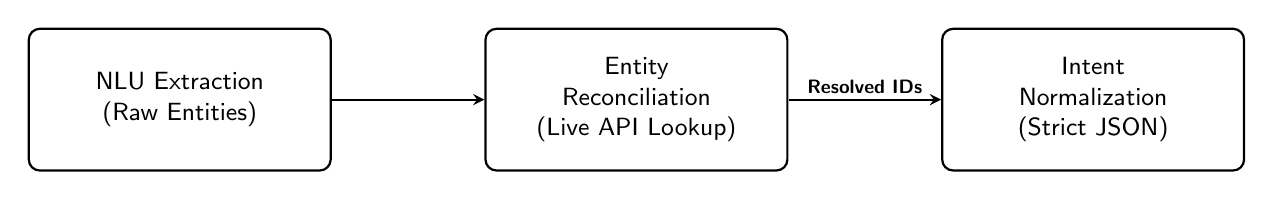
\begin{tikzpicture}[
        node distance=2.5cm,
        every node/.style={font=\sffamily\small},
        procstep/.style={rectangle, draw=black, thick, fill=white, text width=3.6cm, align=center, minimum height=1.8cm, rounded corners},
        arrow/.style={->, thick, draw=black, >=stealth},
        badge/.style={fill=white, font=\sffamily\scriptsize\bfseries, inner sep=2pt}
        ]
        
        % Symmetrical Widened Box Placements (5.8cm center-to-center distance)
        \node[procstep] (nlu) at (0, 0) {NLU Extraction\\(Raw Entities)};
        \node[procstep] (recon) at (5.8, 0) {Entity\\Reconciliation\\(Live API Lookup)};
        \node[procstep] (norm) at (11.6, 0) {Intent\\Normalization\\(Strict JSON)};
        
        % Clean Arrow Connections with Cohesive Masked Badges
        \draw[arrow] (nlu) -- (recon);
        \draw[arrow] (recon) -- node[above, pos=0.5, badge] {Resolved IDs} (norm);
        
    \end{tikzpicture}
    \caption{Entity Grounding and Live Reconciliation Pipeline}
    \label{fig:grounding_pipeline}
\end{figure}

\begin{algorithm}[H]
\caption{Dynamic Entity Grounding and Reconciliation}\label{alg:grounding}
\let\AND\undefined
\let\OR\undefined
\let\NOT\undefined
\begin{algorithmic}[1]
\REQUIRE $I_{\text{raw}}$ (Parsed Raw NLU Intent), $F_{\text{state}}$ (Live Firewall State Query)
\ENSURE $I_{\text{grounded}}$ (Grounded Target Intent) or $E_{\text{error}}$ (Grounding Ambiguity)
\STATE $O_{\text{interfaces}} \leftarrow \text{FetchLiveInterfaces}(F_{\text{state}})$
\STATE $O_{\text{addresses}} \leftarrow \text{FetchLiveAddresses}(F_{\text{state}})$
\FOR{each $E_{\text{entity}}$ in $I_{\text{raw}}.\text{entities}$}
    \STATE $S_{\text{match}} \leftarrow \emptyset$
    \FOR{each $O_{\text{obj}}$ in $O_{\text{interfaces}} \cup O_{\text{addresses}}$}
        \STATE $Score \leftarrow \text{ComputeLevenshteinRatio}(E_{\text{entity}}.\text{name}, O_{\text{obj}}.\text{name})$
        \IF{$Score \ge \text{Threshold } (0.85)$}
            \STATE $S_{\text{match}} \leftarrow S_{\text{match}} \cup \{O_{\text{obj}}\}$
        \ENDIF
    \ENDFOR
    \IF{$|S_{\text{match}}| == 1$}
        \STATE $I_{\text{grounded}}.\text{entities} \leftarrow I_{\text{grounded}}.\text{entities} \cup \{S_{\text{match}}[0]\}$
    \ELSIF{$|S_{\text{match}}| > 1$}
        \RETURN $E_{\text{error}}$ (``Ambiguous reference: multiple matches found'')
    \ELSE
        \STATE $I_{\text{grounded}}.\text{entities} \leftarrow I_{\text{grounded}}.\text{entities} \cup \text{CreateNewObjectPlaceholder}(E_{\text{entity}})$
    \ENDIF
\ENDFOR
\RETURN $I_{\text{grounded}}$
\end{algorithmic}
\end{algorithm}

\subsection{Operational Request Lifecycle}
The orchestration platform is architected as a sequential state machine. Every mutation request traverses a rigorous operational lifecycle designed to enforce security policies and maintain configuration integrity seamlessly.

\begin{table}[H]
    \centering
    \caption{Lifecycle Phases of the Operational Request Pipeline}
    \label{tab:pipeline_phases}
    \renewcommand{\arraystretch}{1.5}
    \small
    \begin{tabular}{|l|p{10.5cm}|}
        \hline
        \textbf{Pipeline Phase} & \textbf{Engineering Responsibility} \\
        \hline
        1. Ingestion & Normalizing multi-turn conversations and maintaining session context. \\
        \hline
        2. Routing & Segregating API reads, RAG queries, and infrastructure mutations. \\
        \hline
        3. Grounding & Extracting configuration parameters and reconciling network entities. \\
        \hline
        4. Validation & Deterministic syntactic and semantic checking of the proposed state. \\
        \hline
        5. HITL Review & Presenting the exact execution diff for explicit administrator authorization. \\
        \hline
        6. Pre-Execution & Capturing the live configuration baseline (snapshot) prior to modification. \\
        \hline
        7. Orchestration & Dispatching serialized REST API payloads to the target FortiGate appliance. \\
        \hline
        8. Verification & Confirming the final operational state securely matches the intended design. \\
        \hline
    \end{tabular}
\end{table}

\section{Security, Compliance, and Transactional Validation}
Once an intent is fully grounded and translated, it is routed to the deterministic validation pipeline in the control plane before reaching the firewall API.

Before any configuration payload reaches the execution layer, it is subjected to multi-tiered validation. The \textbf{Validation Engine} enforces structural integrity, ensuring that IP addresses conform to proper CIDR notations and port definitions align perfectly with standard protocols. Concurrently, the \textbf{Compliance Engine} evaluates the administrative intent against strict organizational security postures.

\begin{table}[H]
    \centering
    \caption{Multi-Tiered Validation and Security Enforcement Layers}
    \label{tab:validation_stages}
    \renewcommand{\arraystretch}{1.5}
    \small
    \begin{tabular}{|l|l|p{6.5cm}|}
        \hline
        \textbf{Validation Tier} & \textbf{Mechanism} & \textbf{Operational Focus} \\
        \hline
        \textbf{Syntactic Layer} & Regex \& Type Checking & Validating IP formats, protocol numbers, and API schema adherence. \\
        \hline
        \textbf{Semantic Layer} & Entity Reconciliation & Ensuring requested objects and policy IDs exist dynamically on the firewall. \\
        \hline
        \textbf{Compliance Layer} & Policy Ruleset Evaluation & Proactively preventing least-privilege violations (e.g., blocking 0.0.0.0/0 on SSH). \\
        \hline
    \end{tabular}
\end{table}


\subsection{Proactive Compliance and Safety Engine}
The \texttt{agent/compliance.py} module implements a rule-based validation engine that enforces security best practices, protecting the enterprise perimeter from accidental administrative misconfigurations. 

We represent a planned firewall policy mutation as $P$, defined by:
\begin{equation}
    P = \langle S_{\text{addr}}, D_{\text{addr}}, Src_{\text{intf}}, Dst_{\text{intf}}, Serv, Act \rangle
\end{equation}
Where $S_{\text{addr}}$ is the source address, $D_{\text{addr}}$ is the destination address, $Src_{\text{intf}}$ is the source interface, $Dst_{\text{intf}}$ is the destination interface, $Serv$ is the list of permitted services, and $Act \in \{\text{accept}, \text{deny}\}$ is the policy action. These compliance filters are implemented as deterministic check methods inside the \texttt{agent/compliance.py} module, executing static validation rules before any REST API update is prepared.

The compliance engine enforces three core validation safety checks:
\begin{enumerate}
    \item \textbf{Implicit Deny Enforcement (Any-to-Any Accept Prevention):}
    If the planned policy permits traffic, it must not apply to global wildcards on both interfaces simultaneously:
    \begin{equation}
        P_{\text{valid}} \implies \neg \big( (Act = \text{accept}) \land (Src_{\text{intf}} = \text{"any"}) \land (Dst_{\text{intf}} = \text{"any"}) \big)
    \end{equation}
    Violations of this rule trigger an immediate safety block within the compliance validator, throwing an exception and halting the orchestrator.
    
    \item \textbf{Insecure Interface Protocol Blocking:}
    Let $I_{\text{protocols}}$ represent the administrative access protocols enabled on a target management interface. The system must prevent binding insecure legacy protocols:
    \begin{equation}
        Access_{\text{valid}} \implies (I_{\text{protocols}} \cap \{\text{"HTTP"}, \text{"TELNET"}\} = \emptyset)
    \end{equation}
    If an operator attempts to enable these protocols on any interface, the validation engine rejects the transaction.
    
    \item \textbf{Insecure Port Public Exposure Prevention:}
    Let $Serv_{\text{ports}}$ represent the TCP/UDP ports mapped to a policy. If a policy bridges a public interface (WAN) to an internal subnet, it must not expose highly vulnerable legacy services (such as SMB or RDP):
    \begin{equation}
        Exposure_{\text{valid}} \implies \Big( Src_{\text{intf}} \in \text{WAN} \implies (Serv_{\text{ports}} \cap \{137, 138, 139, 445, 3389\} = \emptyset) \Big)
    \end{equation}
\end{enumerate}

\subsection{Session Context and Conceptual State Transitions}
To maintain state consistency during multi-turn interactions (such as clarifications or awaiting administrative confirmation), the orchestrator manages a conceptual session lifecycle. Rather than relying on a strict, hardware-bound finite state machine (FSM) implementation, this state machine represents the logical, session-driven context transitions managed dynamically by the \texttt{AgentSession} class. These conceptual states and their permitted transitions are illustrated in Figure~\ref{fig:state_machine}.

To enable robust interaction, the system supports clarification continuity and partial intent persistence. When the user provides an incomplete or ambiguous intent (e.g., "Allow HTTP access" without specifying a destination address), the system transitions to the \texttt{CLARIFY} state. The partial parameters are persisted in memory within the \texttt{SessionContext} class (implemented in \texttt{agent/session\_context.py}). Upon the next user turn, the input is merged with the existing context and re-grounded, ensuring deterministic multi-turn validation without forcing the administrator to restart the command sequence.

\begin{figure}[H]
    \centering
    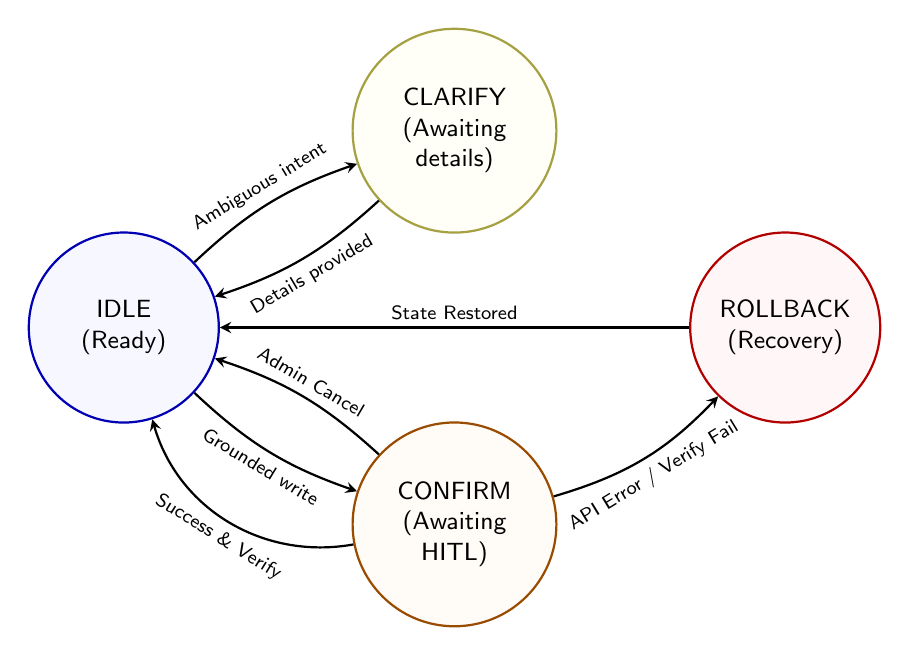
\begin{tikzpicture}[
        node distance=3.0cm,
        every node/.style={font=\sffamily\small},
        stateidle/.style={circle, draw=blue!70!black, thick, fill=blue!3, text width=2.0cm, align=center, minimum height=2.0cm},
        stateclarify/.style={circle, draw=yellow!60!black, thick, fill=yellow!3, text width=2.0cm, align=center, minimum height=2.0cm},
        stateconfirm/.style={circle, draw=orange!60!black, thick, fill=orange!3, text width=2.0cm, align=center, minimum height=2.0cm},
        staterollback/.style={circle, draw=red!70!black, thick, fill=red!3, text width=2.0cm, align=center, minimum height=2.0cm},
        arrow/.style={->, thick, draw=black, >=stealth}
        ]
        
        \node[stateidle] (idle) at (0, 0) {IDLE\\(Ready)};
        \node[stateclarify] (clarify) at (4.2, 2.5) {CLARIFY\\(Awaiting\\details)};
        \node[stateconfirm] (confirm) at (4.2, -2.5) {CONFIRM\\(Awaiting\\HITL)};
        \node[staterollback] (rollback) at (8.4, 0) {ROLLBACK\\(Recovery)};
        
        \draw[arrow] (idle) to[bend left=12] node[above, sloped, font=\sffamily\scriptsize] {Ambiguous intent} (clarify);
        \draw[arrow] (clarify) to[bend left=12] node[below, sloped, font=\sffamily\scriptsize] {Details provided} (idle);
        
        \draw[arrow] (idle) to[bend right=12] node[below, sloped, font=\sffamily\scriptsize] {Grounded write} (confirm);
        \draw[arrow] (confirm) to[bend right=12] node[above, sloped, font=\sffamily\scriptsize] {Admin Cancel} (idle);
        
        \draw[arrow] (confirm) to[bend right=15] node[below, sloped, font=\sffamily\scriptsize] {API Error / Verify Fail} (rollback);
        \draw[arrow] (confirm) to[bend left=42] node[below, sloped, font=\sffamily\scriptsize] {Success \& Verify} (idle);
        \draw[arrow] (rollback) to node[above, font=\sffamily\scriptsize, fill=white, inner sep=2.5pt] {State Restored} (idle);
        
    \end{tikzpicture}
    \caption{State Transition Diagram for multi-turn Administrator Sessions}
    \label{fig:state_machine}
\end{figure}

This session lifecycle manages the safety invariant that the session context cannot transition from \texttt{IDLE} directly to a device mutation without systematically transitioning through the validated and operator-reviewed \texttt{CONFIRM} state.

\subsection{Lifecycle Management \& Transactional Recovery}
To maintain database and network state alignment, the orchestrator encapsulates mutations within a \textbf{Transactional Execution Loop}, implementing a strict try-verify-rollback strategy:
\begin{enumerate}
    \item \textbf{Pre-Mutation Snapshot:} Captures the target configuration parameters (e.g., current ruleset ordering, specific policy parameters) and stores them in a localized stack buffer managed by the \texttt{SnapshotStore} class (\texttt{agent/snapshot.py}).
    \item \textbf{Atomic Execution:} Applies the API changes directly to the FortiOS REST endpoint. The REST client enforces a strict 5-second timeout window; connections exceeding this threshold are aborted to prevent session hanging.
    \item \textbf{Active State Verification:} Immediately issues a post-write query to read back the active state. If the returned state does not match the expected state delta, or if a connection loss occurs (monitored by HTTP heartbeat pings), the system marks the transaction as failed.
    \item \textbf{Inverse Rollback:} Restores the pre-mutation parameters captured in the snapshot, reverting the firewall to its last known stable state.
\end{enumerate}

\subsubsection{Operational Recovery Boundaries and Limitations}
While the transactional loop mitigates deployment risks, physical networking constraints introduce specific operational boundaries:
\begin{itemize}
    \item \textbf{Rollback Connectivity Dependency}: If a configuration mutation inadvertently severs the physical network interface or administrative IP access used by the orchestrator (e.g., changing the management gateway to an unreachable route), the orchestrator will be unable to transmit the inverse rollback payload. In this scenario, the system flags a high-priority alarm on the console and halts, requiring manual physical or out-of-band console recovery.
    \item \textbf{State Persistence Boundaries}: The snapshot buffer writes state directly to local disk (\texttt{logs/snapshots.json}) prior to any mutation. This guarantees that even if the management client or container crashes during execution, the rollback state survives and can be explicitly restored upon system recovery.
\end{itemize}

This fail-safe validation and rollback process is visually modeled in Figure~\ref{fig:verification_workflow}.

\begin{figure}[H]
    \centering
    \begin{tikzpicture}[
        node distance=2.2cm,
        every node/.style={font=\sffamily\small},
        action/.style={rectangle, draw=black, thick, fill=white, text width=2.8cm, align=center, minimum height=1.0cm, rounded corners},
        decision/.style={diamond, draw=black, thick, fill=white, text width=1.8cm, align=center, aspect=1.2},
        arrow/.style={->, thick, draw=black, >=stealth}
        ]
        
        \node[action] (snap) at (0, 0) {Baseline\\Snapshot};
        \node[action] (exec) at (4.5, 0) {API\\Orchestration};
        \node[action] (ver) at (9.0, 0) {State\\Verification};
        \node[decision] (check) at (9.0, -2.5) {Match?};
        
        \node[action] (rollback) at (4.5, -2.5) {Execute\\Rollback};
        \node[action] (commit) at (12.5, -2.5) {Confirm\\Success};
        
        \draw[arrow] (snap) -- (exec);
        \draw[arrow] (exec) -- (ver);
        \draw[arrow] (ver) -- (check);
        \draw[arrow] (check) -- node[above] {No} (rollback);
        \draw[arrow] (check) -- node[above] {Yes} (commit);
        
        % Horizontal-vertical restore line routing back cleanly to Baseline Snapshot bottom edge
        \draw[arrow, dashed] (rollback.west) -- (0, -2.5) -- node[left, pos=0.8] {Restore} (snap.south);
        
    \end{tikzpicture}
    \caption{Transactional Verification and Lifecycle Management Workflow}
    \label{fig:verification_workflow}
\end{figure}

\subsection{Structured Audit and Integrity Logging}
To ensure all configuration changes are completely auditable and detectable against local tampering, the logging component writes transaction logs using a structured rolling hash chain. Each transaction record $T_n$ is chained to the preceding record $T_{n-1}$ by computing:
\begin{equation}
    H(T_n) = \text{SHA-256}\big(T_n.\text{payload} \mathbin{\Vert} H(T_{n-1})\big)
\end{equation}
This validation formula, implemented in our audit logging wrapper, ensures that any unauthorized manual edits to the local log files in \texttt{logs/audit.jsonl} immediately invalidate the sequential hash sequence. It provides local integrity verification for audit trails rather than absolute cryptographic non-repudiation or blockchain-grade guarantees.

\section{UML Use Case and Structural Modeling}
To map the active interfaces and object relationships that control the transactional pipeline, we provide formal Unified Modeling Language (UML) notations of the system.

The interaction boundaries between the system operator (network administrator), the hybrid orchestration agent, and the physical FortiGate firewall are modeled in the global Use Case diagram shown in Figure~\ref{fig:uml_use_case}.

\begin{figure}[H]
    \centering
    \begin{tikzpicture}[
        scale=0.85, every node/.style={transform shape},
        actorhead/.style={draw=blue!70!black, thick, circle, minimum size=0.6cm, fill=blue!5},
        firewallbox/.style={draw=orange!70!black, thick, rectangle, minimum width=0.9cm, minimum height=0.9cm, rounded corners, fill=orange!5},
        usecase/.style={draw=blue!70!black, thick, ellipse, minimum width=3.4cm, minimum height=1.0cm, align=center, fill=white, font=\sffamily\small},
        systembox/.style={draw=gray!50, thick, rectangle, minimum width=9.5cm, minimum height=12.2cm, fill=gray!5, rounded corners},
        arrow/.style={-, thick, draw=black},
        include/.style={->, dashed, thick, draw=black, >=stealth, font=\sffamily\scriptsize}
        ]
        
        % Boundaries \& System Container
        \node[systembox] (sys) at (5.0, -5.7) {};
        %\node[font=\sffamily\small\bfseries\color{gray!80}] at (5.0, -0.0) {FortiGate Orchestrator Boundary};
        
        % Operator Actor (Stick Figure Head)
        \node[actorhead] (admin) at (-2.0, -5.0) {};
        % Stick Figure Body \& Limbs
        \draw[thick, draw=blue!70!black] (admin.south) -- ++(0, -0.6) coordinate (torso);
        \draw[thick, draw=blue!70!black] (torso) -- ++(-0.3, -0.5);
        \draw[thick, draw=blue!70!black] (torso) -- ++(0.3, -0.5);
        \draw[thick, draw=blue!70!black] (admin.south) ++(0, -0.15) -- ++(-0.4, 0.1);
        \draw[thick, draw=blue!70!black] (admin.south) ++(0, -0.15) -- ++(0.4, 0.1);
        \node[font=\sffamily\small\bfseries] at (-2.0, -6.6) {Administrator};
        
        % Firewall Device Actor (Server Rack Representation)
        \node[firewallbox] (fw) at (12.0, -5.2) {};
        \draw[thick, draw=orange!70!black] (11.65, -5.05) -- (12.35, -5.05);
        \draw[thick, draw=orange!70!black] (11.65, -5.35) -- (12.35, -5.35);
        \fill[orange!70!black] (11.8, -5.05) circle (0.04cm);
        \fill[orange!70!black] (11.8, -5.35) circle (0.04cm);
        \node[font=\sffamily\small\bfseries] at (12.0, -6.0) {FortiGate Firewall};
        
        % Use Cases inside boundary
        \node[usecase] (uc1) at (5.0, -1.5) {Query System State\\(Read-Only RAG)};
        \node[usecase] (uc2) at (5.0, -4.5) {Modify Security Configuration\\(Conversational Intent)};
        \node[usecase] (uc3) at (5.0, -7.5) {Review Staged Delta Diff\\(HITL Portal)};
        \node[usecase] (uc4) at (5.0, -10.5) {Perform Transactional Rollback\\(Recovery Stack)};
        
        % Administrative Links (connected to head node)
        \draw[arrow] (admin) -- (uc1);
        \draw[arrow] (admin) -- (uc2);
        \draw[arrow] (admin) -- (uc3);
        
        % Firewall Links (connected to firewall node)
        \draw[arrow] (uc1) -- (fw);
        \draw[arrow] (uc2) -- (fw);
        \draw[arrow] (uc4) -- (fw);
        
        % Dependencies (includes \& extends)
        \draw[include] (uc2) -- node[right, fill=gray!5, inner sep=1.5pt] {\footnotesize\textit{<<include>>}} (uc3);
        \draw[include] (uc4) -- node[right, fill=gray!5, inner sep=1.5pt] {\footnotesize\textit{<<extend>>}} (uc2);
        
    \end{tikzpicture}
    \caption{UML Use Case Diagram representing Operator Interactions and System Boundaries}
    \label{fig:uml_use_case}
\end{figure}

The structural design of the Python backend is modeled in the UML Class Diagram shown in Figure~\ref{fig:uml_class_diagram}. This diagram illustrates the properties, methods, and relationships of the active modules.

\begin{figure}[H]
    \centering
    \begin{tikzpicture}[
        scale=0.85, every node/.style={transform shape},
        classbox/.style={rectangle, draw=blue!70!black, thick, fill=blue!3, text width=5.7cm, align=left, rounded corners, font=\sffamily\scriptsize, inner sep=6pt},
        dataclassbox/.style={rectangle, draw=purple!70!black, thick, fill=purple!3, text width=5.7cm, align=left, rounded corners, font=\sffamily\scriptsize, inner sep=6pt},
        arrow/.style={->, thick, draw=black, >=stealth},
        dependency/.style={->, thick, dashed, draw=black, >=stealth},
        composition/.style={{Diamond[black]}-, thick, draw=black, >=stealth}
        ]
        
        % Class 1: AgentSession
        \node[classbox] (session) at (0, 0) {
            {\centering\textbf{AgentSession}\par}\vspace{0.08cm}
            {\color{blue!30!black}\rule{\linewidth}{0.4pt}}\\[0.12cm]
            - conversation: list\\
            - \_pending: ConfirmationState\\
            - ctx: SessionContext\\
            - snapshots: SnapshotStore\\[0.12cm]
            {\color{blue!30!black}\rule{\linewidth}{0.4pt}}\\[0.12cm]
            + process(user\_input: str): AgentResponse\\
            + has\_pending(): bool\\
            + \_route(user\_input: str): AgentResponse
        };
        
        % Class 2: RawIntentSchema
        \node[dataclassbox] (nlu) at (7.2, 3.2) {
            {\centering\guillemotleft dataclass\guillemotright\\ \textbf{RawIntentSchema}\par}\vspace{0.08cm}
            {\color{purple!30!black}\rule{\linewidth}{0.4pt}}\\[0.12cm]
            + intent: NLUIntentType\\
            + confidence: NLUConfidence\\
            + policy\_ids: List[int]\\
            + is\_multi\_policy: bool\\
            + deltas: List[NLUDelta]\\
            + policy\_filter: dict\\
            + raw\_input: str\\
            + missing\_fields: List[str]\\[0.12cm]
            {\color{purple!30!black}\rule{\linewidth}{0.4pt}}\\[0.12cm]
            + is\_complete(): bool
        };
        
        % Class 3: GroundedIntentSchema
        \node[dataclassbox] (grounder) at (7.2, -3.2) {
            {\centering\guillemotleft dataclass\guillemotright\\ \textbf{GroundedIntentSchema}\par}\vspace{0.08cm}
            {\color{purple!30!black}\rule{\linewidth}{0.4pt}}\\[0.12cm]
            + raw: RawIntentSchema\\
            + policy\_ids: List[int]\\
            + current\_state: dict\\
            + grounded\_deltas: List[NLUDelta]\\
            + is\_valid: bool\\
            + is\_noop: bool\\
            + noop\_message: str\\
            + issues: List[GroundingIssue]\\
            + computed: dict\\[0.12cm]
            {\color{purple!30!black}\rule{\linewidth}{0.4pt}}\\[0.12cm]
            + error\_messages(): List[str]
        };
        
        % Class 4: SnapshotStore
        \node[classbox] (snapshot) at (14.4, 3.2) {
            {\centering\textbf{SnapshotStore}\par}\vspace{0.08cm}
            {\color{blue!30!black}\rule{\linewidth}{0.4pt}}\\[0.12cm]
            - \_snapshots: deque\\[0.12cm]
            {\color{blue!30!black}\rule{\linewidth}{0.4pt}}\\[0.12cm]
            + capture(tool, resource, state, desc, fn): str\\
            + list(): List[OperationSnapshot]\\
            + get(op\_id: str): OperationSnapshot\\
            + mark\_rolled\_back(op\_id: str)\\
            + format\_list(): str
        };
        
        % Class 5: PolicyUpdateExecutor
        \node[classbox] (executor) at (14.4, -3.2) {
            {\centering\textbf{PolicyUpdateExecutor}\par}\vspace{0.08cm}
            {\color{blue!30!black}\rule{\linewidth}{0.4pt}}\\[0.12cm]
            - \_get: function\\
            - \_update: function\\
            - \_READONLY\_FIELDS: set\\[0.12cm]
            {\color{blue!30!black}\rule{\linewidth}{0.4pt}}\\[0.12cm]
            + execute(intent: UpdateIntent): ExecResult\\
            - \_fetch(policy\_id: int): dict\\
            - \_check\_noops(current: dict, deltas: list)\\
            - \_apply\_deltas(target: dict, deltas: list)
        };
        
        % Relationships
        \draw[dependency] (session) -- (nlu);
        \draw[dependency] (session) -- (grounder);
        \draw[dependency] (grounder) -- (executor);
        \draw[dependency] (executor) -- (snapshot);
        \draw[composition] (session.north) -- ++(0, 2.4) -| (snapshot.north);
        
    \end{tikzpicture}
    \caption{UML Class Diagram representing structural relationships of Python Backend Classes}
    \label{fig:uml_class_diagram}
\end{figure}

The `AgentSession` context class acts as the central coordinator, orchestrating transitions between the conversational NLU layers and the deterministic components. The dynamic NLU parsing yields `RawIntentSchema` instances, which are immediately directed to the grounding engine to produce verified `GroundedIntentSchema` structures. Finally, mutations are managed by the `PolicyUpdateExecutor` coupled with the transactional recovery capabilities of the `SnapshotStore` to ensure fail-safe operation on the physical firewall appliance.

\section{Chapter Conclusion}
This chapter has detailed the architectural design, ingestion pipelines, and structural specifications of the hybrid network orchestration prototype. By segregating the system into a probabilistic interpretation plane and a deterministic control plane, we enforce a strict trust boundary. We have modeled the NLP \& RAG enrichment stages, established functional diagrams using UML Use Cases, defined the detailed software components using class models, and mathematically formulated the safety gates that enforce corporate security postures. These designs establish a highly precise, verifiable blueprint for secure network automation.